\documentclass{article}
\usepackage[utf8]{inputenc}
\setlength{\parindent}{0pt}
\addtolength{\hoffset}{-3cm}
\addtolength{\textwidth}{6cm}
\usepackage[francais]{babel}
\usepackage{fontspec}
\usepackage{amsmath}
\usepackage{amsfonts}
\usepackage{xcolor,graphicx}
\usepackage{minted}
\usemintedstyle{colorful}
\usepackage{float}

\title{Kernel TP3 - Rapport système de fichiers - TexFS}
\author{Maxime Lovino \and Loic Willy}

\begin{document}
\maketitle
\newpage
\section{Introduction}
Pour réaliser le système de fichiers utilisé par notre Kernel, nous nous sommes inspirés du système de fichiers Ext2 sur lequel nous avons travaillé pendant un semestre en deuxième année. Nous avons adapté Ext2 par rapport aux besoins qui étaient spécifiés pour ce projet. C'est-à-dire que nous avons principalement simplifié Ext2 en supprimant les doubles et triples indirections, qui ne sont pas nécessaires compte tenu de la taille des fichier que nous devons stocker. Nous n'avons également pas tenu compte de la notion de groupes.\\

De ce fait, lors de la création d'une image TexFS, il est nécessaire de spécifier la taille de bloc, le nombre de bloc à allouer et le nombre de fichiers maximum pour l'image. La taille de bloc et le nombre de blocs devaient être spécifiés de toute façon, mais compte tenu de la structure utilisée, il est nécessaire d'entrer également le nombre de fichiers maximum que contiendra l'image. (Si nous avions des groupes, nous aurions pu allouer un nouveau groupe en cas de besoins de nouveaux fichiers)
\section{Structure du système de fichiers}
\begin{figure}[H]
    \centering
    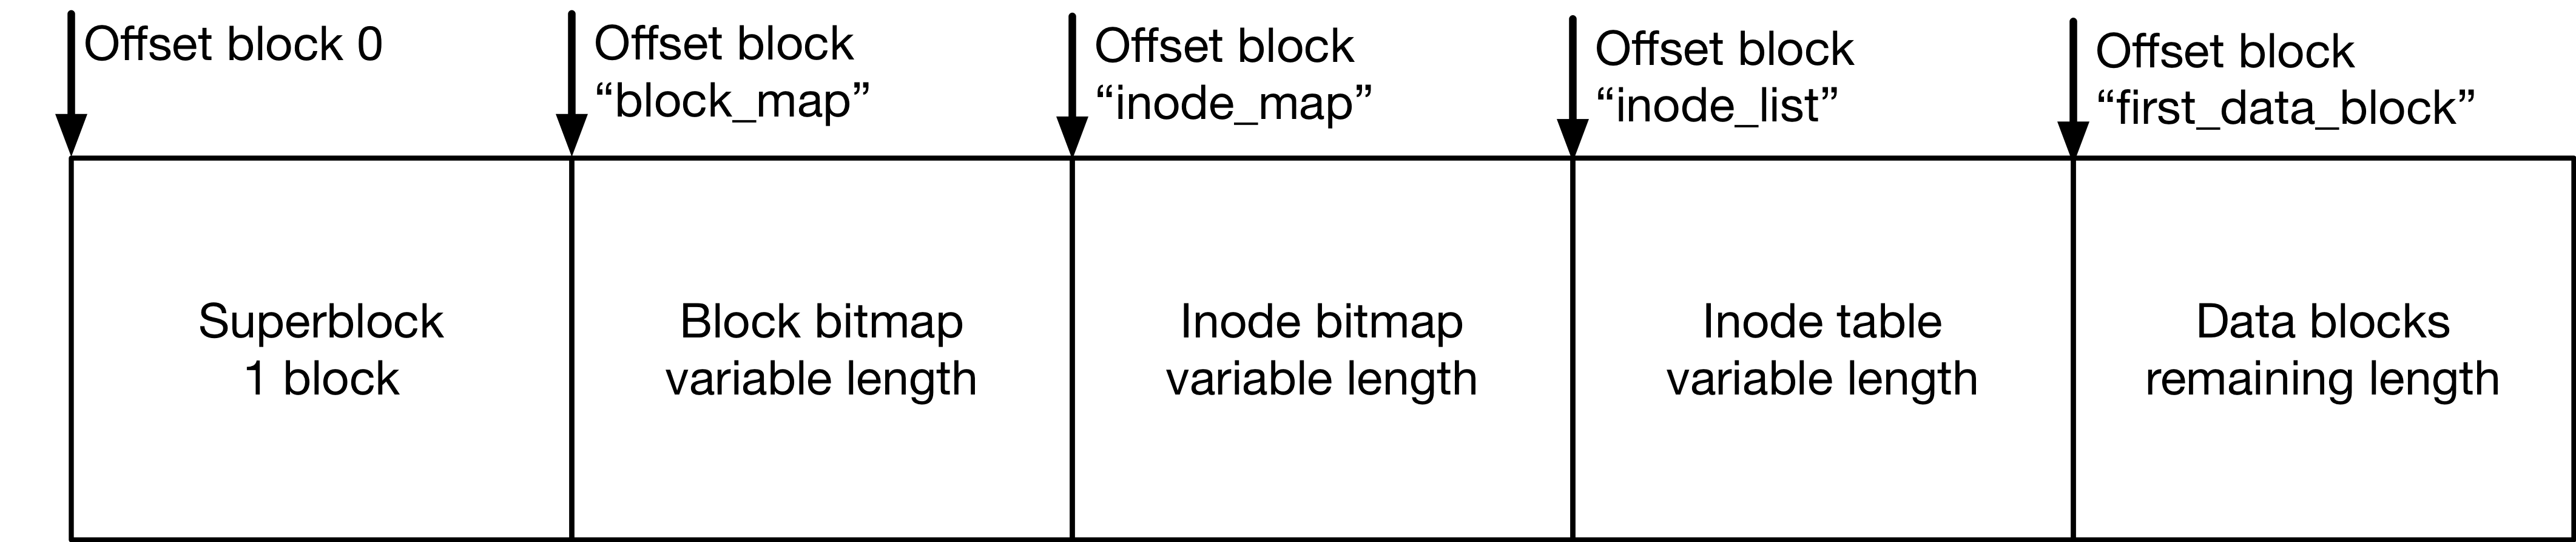
\includegraphics[width=\textwidth]{FS_disk_structure.png}
\end{figure}
\subsection{Blocs de métadonnées}
\subsubsection{Superblock}
\begin{minted}[breaklines,breaksymbol=, linenos, frame=single, stepnumber=5,tabsize=2]{C}
typedef struct tex_fs_superblock_st {
    uint16_t magic;
    uint8_t version;
    char label[MAX_LABEL_LENGTH];
    uint16_t block_size;
    uint32_t block_map;
    uint32_t block_count;
    uint32_t inode_bitmap;
    uint32_t inode_list;
    uint32_t inode_count;
    uint32_t first_data_block;
} __attribute__((packed)) tex_fs_superblock_t;	
\end{minted}
\subsubsection{Block bitmap}
\subsubsection{Inode bitmap}
\subsubsection{Inode Table}
\begin{minted}[breaklines,breaksymbol=, linenos, frame=single, stepnumber=5,tabsize=2]{C}
typedef struct tex_fs_inode_st {
    char name[MAX_FILENAME_LENGTH];
    uint32_t size;
    uint32_t direct_blocks[DIRECT_BLOCKS];
    uint32_t indirect_blocks[INDIRECT_BLOCKS];
} __attribute__((packed)) tex_fs_inode_t;
\end{minted}

\section{Exemples}
\section{Implémentation}
\section{Avantages du système choisi}
\section{Inconvénients du système choisi}
\end{document}
